\section{Face Detection} \label{section:fd}
Face detection is a computer vision task that involves locating one or multiple human faces in an image or video. It has been an active area of research in computer vision for several decades. Over the years, various methods have been proposed to address this problem, ranging from simple heuristic-based techniques to sophisticated machine learning algorithms \cite{feng_detect_2022}.

Lubna Aziz et al. \cite{aziz_exploring_2020} emphasizes deep learning's application in areas like surveillance, transportation, and medicine, considering challenges like object variety and limited computational resources. Over the years, the trend has moved from handcrafted feature-based methods to data-driven machine learning methods, and currently, deep learning-based approaches dominate the field due to their superior performance.

``Fig.~\ref{od-timeline}'' provides a overview of how the Generic Object Detection and Face Detection landscape has changed over the years. One can see before 2012 the algorithms used some sort of manual feature extraction method but after 2012 the deep learning based methods started becoming the State of the art (STOA) algorithms. After 2012 on the top branch are the multi stage based Face Detection models while on the bottom are the single stage based Face detection models, in the middle branch are Generic Object detection models which are considered more challenging than face detection.

\begin{figure}[htbp]
\centerline{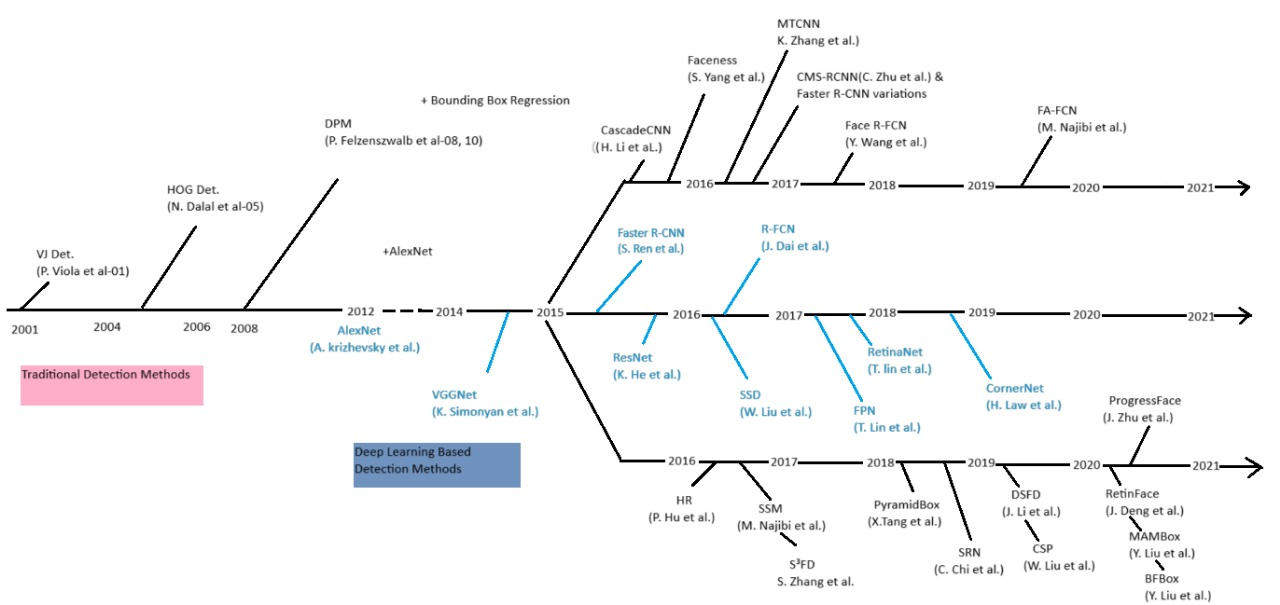
\includegraphics[width=\columnwidth]{assets/od-timeline.jpg}}
\caption{Object Detection and Face Detection Timeline Overview}
\label{od-timeline}
\end{figure}

Several methods and frameworks, like Viola-Jones \cite{sumanto_viola-jones_2022}, \cite{rani_face_2022}, HOG \cite{rani_face_2022}, MTCNN \cite{rani_face_2022}, MobileNet-SSD \cite{chan_face_2022}, and YOLO-Face \cite{wang_yolov5s-face_2022}, have been utilized to ensure consistent face detection in varying conditions. Once the face is extracted, recognition involves comparing faces within a certain range or threshold, with techniques like PCA and ICA used for accuracy. Lightweight model advancements, such as those based on lightweight models like GhostNet \cite{alansari_ghostfacenets_2023}, have also been explored to meet computational demands for lower end devices.

Authors in \cite{sumanto_viola-jones_2022} used ViolaJones method's on WIDER FACES dataset and achieved a 100\% success rate on detection in groups and meetings, while the previous approaches only managed the highest accuracy results were obtained at 90.9\% for facial images and 75.5\% for non-face images. While these approaches are good under controlled environments their accuracy decreases in uncontrolled environments. Exploring the challenges of detecting faces in uncontrolled environments with varying poses, addressing shortcomings caused by environmental factors, lighting conditions, and image quality authors in \cite{mahesh_smart_2022} proposed an 8-layer Alexnet Convolutional Neural Network (ACNN). By comparing ACNN with the Support Vector Machine (SVM), the research demonstrates that ACNN outperforms SVM, achieving a remarkable 96\% accuracy compared to SVM's 89\% in recognizing faces with varying poses.

Multitask-Net model proposed in \cite{viet_simultaneous_2021} overcomes the challenges of face detection and head pose estimation in digital images which is vital for applications like surveillance. The authors enhances head pose estimation accuracy by leveraging features from face detection and predicts head position and direction simultaneously, utilizing Rotation matrix vectors for face orientation representation to overcome limitations. The results showcase the model's high accuracy, comparable to state-of-the-art methods.

Addressing the issues of missed and false face detection Yongwang Wand et al. \cite{wang_yolov5s-face_2022} proposed a new model based on YOLOV5s by modifying the anchor box size using K-means clustering, embedding an SE attention module on the backbone of YOLOV5s and adding four-scale feature detection for small target faces. This new model gained 3.9\% in mAP and 4.0\% in Recall compared to YOLOV5s. In another paper by Aifian Adi Sufian et al. \cite{chan_face_2022} introduces a two-step face detection framework designed to reduce over-detection in face images and misdetection in non-face images. The method combines feature detection using SSD MobileNet V2 and a geometrical algorithm. When compared to leading algorithms the approach achieved a 91.5\% prediction accuracy. Although it didn't surpass MTCNN and Dlib in accuracy, it was superior in minimizing both over-detection and misdetection.

Farooq et al. \cite{farooq_hybrid_2021} highlights the challenges posed by variations in age, lighting, expressions, and image quality, especially for individuals with dark skin, where existing algorithms tend to perform poorly. To address this racial disparity in facial recognition technology, the authors presents a hybrid algorithm combining Gaussian Model and Explicit Rule Algorithm for skin detection. This innovative approach significantly improves the face detection accuracy for dark-skinned individuals by an impressive 89\%. This underscores the importance of diverse training datasets.

Night time video surveillance arising from varying environmental light conditions can lead to underexposed distant objects and overexposed nearby objects. To combat these issues, the authors in \cite{lu_fusion_2022} introduces the concept of a multi-intensity IR illuminator with periodically varying intensity. The MI3 database is established to assess object detectors in different scenes and illuminations. It evaluates human and face detectors, presenting satisfactory results for simple scenes and proposing a baseline approach for fusion among different illumination intensities.

Khalid M et al. \cite{hosny_privacy_2022} addresses the pressing need for privacy protection in surveillance videos, given the ubiquity of surveillance cameras in our lives. It focuses on safeguarding sensitive regions, particularly people's faces, within surveillance footage. The proposed method employs an object detector, YOLOv3 \cite{aziz_exploring_2020}, to identify the regions and subsequently applies a fast block scrambling technique for obfuscation. Encryption is then applied using secret keys generated from a chaotic logistic map. Notably, the method extends protection to the edges of detected regions to prevent sensitive information leakage. This approach offers practical and robust privacy protection for surveillance videos, ensuring the confidentiality of sensitive data and resilience against potential attacks.

While convolutional neural networks (CNNs) or other Deep learning based approaches have shown promise in face detection, their computational demands can be prohibitive, especially for CPU-based systems as it also adds to the computational complexity and thus requires good hardware which is often not the case with real time surveillance systems, the critical need for lightweight and efficient face detection methods without compromising accuracy was addressed by Muhamad Dwisnanto Putro et al \cite{putro_high_2021}. The authors introduces an optimized architecture, featuring a lightweight CNN with two key modules: a feature extraction backbone and a multilevel detector for accommodating scale variations in face detection. This innovative approach achieves state-of-the-art performance among CPU-based real-time detectors, running at an impressive 53 frames per second (FPS), while requiring fewer than one million parameters.